\documentclass[12pt,onecolumn,letterpaper]{article}

\usepackage{cvpr}
\usepackage{times}
\usepackage{epsfig}
\usepackage{graphicx}
\usepackage{amsmath}
\usepackage{amssymb}
\usepackage{subcaption} 
\usepackage[normalem]{ulem}
\useunder{\uline}{\ul}{}
\usepackage{lipsum}
\usepackage{tabularx}
\usepackage{placeins}
\usepackage{float}

\usepackage[breaklinks=true,bookmarks=false]{hyperref}

\cvprfinalcopy 

\def\cvprPaperID{****} % *** Enter the CVPR Paper ID here
\def\httilde{\mbox{\tt\raisebox{-.5ex}{\symbol{126}}}}

\begin{document}

%%%%%%%%% TITLE
\begin{titlepage}
   % \newgeometry{top=25mm,bottom=25mm,left=38mm,right=32mm}
   \setlength{\parindent}{0pt}
   \setlength{\parskip}{0pt}
   % \fontfamily{phv}\selectfont

   {
                   \Large
                   \raggedright
                   Imperial College London\\[17pt]
                   Department of Electrical and Electronic Engineering\\[17pt]
                   Final Year Project Report 2019\\[17pt]
   }

   \rule{\columnwidth}{3pt}
   \vfill
   \centering
     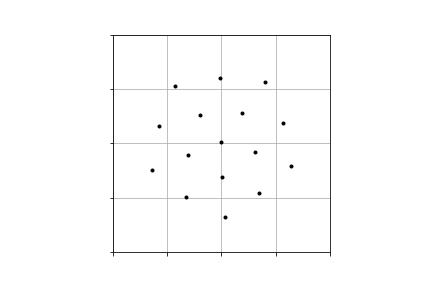
\includegraphics[width=0.7\columnwidth,height=60mm,keepaspectratio]{../figures/cover_photo.png}
   \vfill
   \setlength{\tabcolsep}{0pt}

   \begin{tabular}{p{40mm}p{\dimexpr\columnwidth-40mm}}
                   Project Title: & \textbf{Machine Learning for Communications with Short Block Length} \\[12pt]
                   Student: & \textbf{Alistair P. S. Wallace} \\[12pt]
                   CID: & \textbf{01062642} \\[12pt]
                   Course: & \textbf{EEE4} \\[12pt]
                   Project Supervisor: & \textbf{Dr Bruno Clerckx} \\[12pt]
                   Project Cosupervisor: & \textbf{Dr Morteza Varasteh} \\[12pt]
                   Second Marker: & \textbf{Dr Cong Ling} \\
   \end{tabular}
\end{titlepage}

%%%%%%%%% Contents Page
\tableofcontents
\pagebreak

%%%%%%%%% ABSTRACT
\begin{abstract}   
   This report focused on applying recent developments in machine learning to the field of communications to improve performance over channels which are unknown or difficult to model. It has been shown that optimising each stage of a communication system individually gives suboptimal performance, leading to investigating end-to-end learnt communication systems, where the optimal communication system can be learnt for a particular channel, environment and for specific hardware non-idealities.
   
   The report reproduces results from two recent papers ~\cite{oShea,Aoudia} on the subject, exploring unsupervised models and investigating supervised models with additive white Gaussian noise (AWGN), Rayleigh block fading (RBF). It then goes further by applying the above methods to Ricean fading (RF) channels.
   
   The report produced predominantly similar results to ~\cite{oShea} for supervised models, giving identical performance for two of the three ($n$,$k$) configurations. However, differences were found, sometimes showing lower performance of the technology in question or less aesthetic t-distributed stochastic neighbor embedding (t-SNE) based constellation diagrams, which the original authors overlooked.
\end{abstract}

\FloatBarrier
\section{Introduction}

\subsection{Introduction to the subject}

This project is on machine learning for communications with short block lengths. A typical communication system is shown in Figure \ref{fig:ClassicalCommsBlockDiagram}. As can be seen, it has many discrete modular parts, all of which are optimised individually, however, it has been shown that this gives sub-optimal performance~\cite{ChannelEncodingOptimality}.

\begin{figure}[t]
\begin{center}
   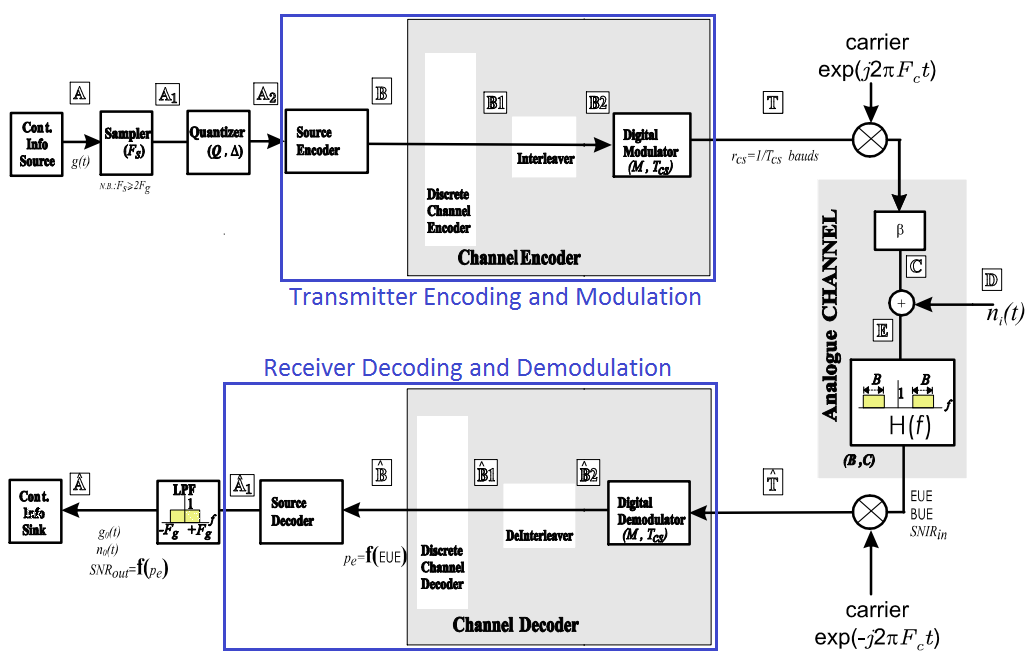
\includegraphics[width=0.8\linewidth]{figures/classical_comms_block_diagram.png}
\end{center}
   \caption{A block diagram of a classical communications system. Taken from ~\cite{EE3CommsSystemsNotesL4}.}
\label{fig:ClassicalCommsBlockDiagram}
\end{figure}

\begin{figure}[t]
\begin{center}
   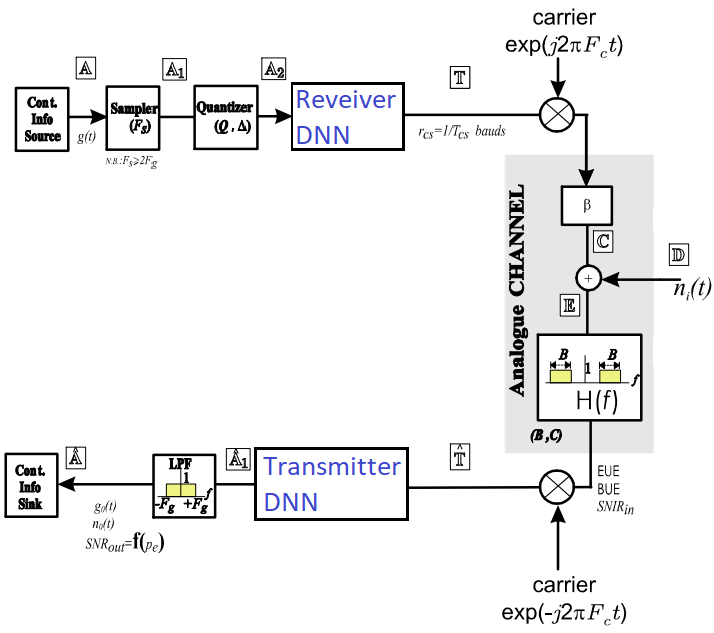
\includegraphics[width=0.8\linewidth]{figures/dnn_block_diagram.png}
\end{center}
   \caption{A block diagram of a DNN based communication system. Based on a diagram from ~\cite{EE3CommsSystemsNotesL4}.}
\label{fig:DNNCommsBlockDiagram}
\end{figure}

The idea of this research is to replace all the individually optimised modules with one deep neural network (DNN) each for the transmitter and receiver. This involves replacing everything within each blue box in Figure \ref{fig:ClassicalCommsBlockDiagram} with one neural network (NN), as is shown in Figure \ref{fig:DNNCommsBlockDiagram}. 

Normally the information goes through two sets of encoding, source encoding to compress the information content, followed by channel encoding to make it robust to channel noise. Whereas using the DNN method all of the communication system's encoding can be learned simultaneously, and the overall communication system can be optimised for hardware non-idealities such as non-linear power amplifiers. It also allows the locally optimal communication system for a given channel to be learnt, without trying to categorise or make assumptions about the channel.

\subsection{Project deliverables}

The main aim of this project is to reproduce the results from two recent papers ~\cite{oShea,Aoudia} on the subject. The secondary deliverable was a potential extra objective for if the project was finished early. This deliverable was left unspecified, but would be to do something new. For instance tackling the limitation of being limited to short block lengths, or investigating potential opportunities such as learning an optimal communication system for a channel which could not be mathematically modelled, or could be modelled but couldn't be solved.

The two papers originally contributed five deliverables, four from the first and one from the second. However the project supervisor advised that only the first deliverable from each paper were important and so only these deliverables were attempted. 

The first paper, by O'Shea \etal~\cite{oShea}, was only the second paper on the subject, following a paper 8 months earlier by one of the same authors~\cite{oShea0}. The O'Shea paper first demonstrated that an end-to-end communication system could be learned in an autoencoder like method, the structure of which can be seen in Figure \ref{fig:oSheaAutoencoderLayout}. 

It trained a range of autoencoders across a range of ($n$,$k$) combinations for which the constellation diagrams and performance over different signal to noise ratios (SNRs). These autoencoders had several different types of regularisations which affected their constellation diagrams. Their performance was compared to non-learned methods of encoding, such as BPSK and QAM for channel encoding and Hamming maximum likelihood and hard decision for source encoding. 

\subsubsection{Side note on autoencoders}

Note that while this would be better suited to the background section, it is necessary for understanding the introduction, so it has been placed here.

Autoencoders are a technique used in deep learning (DL) for encoding and compressing data. There are two NNs placed end-to-end, as in Figure \ref{fig:oSheaAutoencoderLayout}. The input to the first network is $s \in \mathcal{M} = \{1,2,\dots,M\}$, where each $s$ can be represented by $k$ bits. The encoder (first network, analogous to the transmitter), compresses $s$ to $x \in \mathcal{N} = \{1,2,\dots,N\}$, represented by $n$ bits. The decoder (second network, analogous to the receiver) decodes $x$ back to $\hat{s}$.

Normally with autoencoders $n < k$, because the autoencoder is finding a compressed form of $\mathcal{M}$ which maintains the information content, while reducing the number of bits used. However in this paper because there is noise added in middle layer, as shown in Figure \ref{fig:oSheaAutoencoderLayout}, $n \geq k$ to increase robustness of the transmitted signal to noise (minimise information loss).

\subsubsection{Project deliverables continued}

Moving back to the O'Shea paper, it should be noted that all the following deliverables were written off by the project supervisor and so were not attempted, they are just described to give a better understanding of the O'Shea paper. 

The paper then went on to investigate training two adversarial networks, but then showed that this was the same as optimising one multiple input multiple output (MIMO) NN with one common or multiple individual performance metrics. Thirdly the authors introduced radio transformer networks (RTNs) which improved performance of the learned communication system in all cases. Lastly the authors investigated using NNs for modulation classification. All of these sections were competitive with or outperformed current state of the art. 


\begin{figure}[t]
\begin{center}
   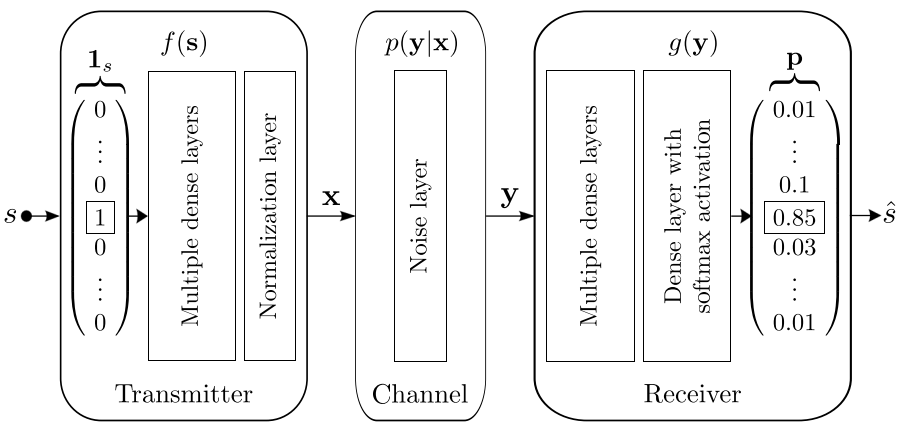
\includegraphics[width=0.8\linewidth]{figures/oShea_autoencoder_layout.PNG}
\end{center}
   \caption{A diagram of the structure of the autoencoder model. Taken from~\cite{oShea}}
\label{fig:oSheaAutoencoderLayout}
\end{figure}

The details of what the paper achieved will be covered in more detail in the background section, however a high level description was needed as reproducing these results were the main deliverables. Each of these sections would require writing some python code and then using this to reproduce the graphs and constellation diagrams. The authors stated that Keras "has become our primary tool used to generate the numerical results for this manuscript"~\cite{oShea}. Consequently Keras has also been used here to reproduce the results.

The second paper by Aoudia and Hoydis improves on the first by removing the need for a differentiable model of the channel. This helps access the technologies' main potential, which is learning general and optimal communication systems for unmodelable or analytically insoluble channels. 

This paper exclusively solved the problem of implementing reinforcement learning to avoid the need for a differentiable channel model. However it should be noted that supervisor advice says this method's implementation is much more difficult and should not be underestimated.

The main twp deliverables are summarised below.

\begin{enumerate}
   \item Make an autoencoder model and compare it's performance to differential binary phase shift key (DBPSK) and Hamming encoding across a range of signal to noise ratios (SNRs)
   \begin{itemize}
      \item Produce complex channel symbolled (2,2) and (8,8) autoencoders, then obtain their constellation diagrams.
      \item Produce non-complex channel symbolled (7,4) autoencoder and obtain a t-SNE dimensionally reduced constellation diagram.
      \item Write encoding and decoding functions for Hamming HD and MLD
      \item Write encoding and decoding functions for BPSK
      \item Compare the performance of various encoding methods and debug until Figures 3a,b from ~\cite{oShea} were reproduced.
   \end{itemize}
   \item Reproduce the unsupervised reinforcement learning model from ~\cite{Aoudia} which uses the alternate training method. The compare the performance of this model against current state of the art and the autoencoder method across a range of SNRs for an AWGN and an RBF channel.
   \begin{itemize}
      \item Produce a custom layer to implement RBF.
      \item Replicate the paper's supervised model for an RBF channel.
      \item Compare AWGN model from previous deliverable's performance across range of SNRs to the results from the paper. Next do the same with new supervised RBF model.
      \item Produce unsupervised model for AWGN channel
      \item Compare performance of AWGN unsupervised model across range of SNRs.
      \item Produce unsupervised model for RBF channel
      \item Compare performance of RBF unsupervised model across range of SNRs.
      \item Once satisfied all four models are performing as they are reported to have in the paper, assess speed of convergence to correct model for all four AWGN, RBF, supervised and unsupervised models.
   \end{itemize}
\end{enumerate}

Any additional work is likely to be one of two options. Either by improving on the work done with reinforcement learning in~\cite{Aoudia}, either tackle the limitations on block lengths, try to improve the convergence time, investigate the systems performance difficult channels or integrating RTNs with the reinforcement learning, as this always improved the results in~\cite{oShea}.

The other option would be to be working on simultaneous wireless information and power transfer (SWIPT) systems. Either investigating the effect of block length on rate-power (RP), obtaining a model that features the practical limitations of the rectenna (rectifier-antenna) used in the EH part, or the dependency between delivered power and channel input average input power.

From assessment of the literature the author thinks that it would be better to look into extending the work of reinforcement learning paper, because it better unlocks the potential of this technology. However the supervisor of the project has informed the author that the he will decide based on which area is developing fastest at the time.  

From a high level, the project is a software project and so the end deliverables will be a series of python scripts and functions which can learn a full end-to-end communication system. Along side these will be documentation of how to use these functions and scripts as well as comparison of the results produced with the results in the paper's the author is reproducing.

There may be customisations which allow it to use optimal formats for different channels, however this detracts slightly from the idea of an adaptable communication system that can learn an optimal communication system for any long term stationary channel.

Because of the nature of the project there will not be any hardware produced, although there will be some analytical work in analysis of channels.

\subsection{Motivation}

Two reasons for looking into this subject are, the recentness of it's discovery and the exceedingly promising results, both within the field of communications and of the underlying technology. These within field results are particularly impressive in a long established field where the improvements have become more marginal in modern times~\cite{oShea}.

Other than the intellectual elegance of a fully learned communication system, there are significant advantages to a fully learned system. 

The first reason is that although for known, ideal, mathematically model-able channels there are often mathematically proven optimal methods, particularly for linear, stationary Gaussian channels. In reality there are many imperfections and non-linearities~\cite{NonLinearities} both in the channel and also in the hardware such as non-linear power amplifiers and finite resolution quantisation. These often cannot be fully accounted for in an analytical solution, leading to sub-optimal performance. Whereas, a fully learned communication system could self-optimise for different hardware configurations and channel environments, with no assumptions about those factors other than stationarity.

Secondly communication systems are normally split into blocks (eg quantisation, modulation, source and channel encoding as shown in Figure \ref{fig:oSheaAutoencoderLayout}). It has been shown that optimising these blocks individually leads to sub-optimal performance, as is shown here in the cases of short block lengths and in use on practical channels~\cite{ChannelEncodingOptimality, NonOptimalRayleigh}.

A third reason to use NNs is that there have been some impressive demonstrations of the learning ability of both feedforward and recurrent NNs (RNNs), suggesting this is a promising area which we should try applying to communications. Recurrent NNs have been shown to be Turing-complete~\cite{RnnTuringComplete} and more recently there has been some very impressive work done on learning algorithms with RNNs~\cite{NeuralProgramInterpreters}. 

More relevantly, but less recently, feedforward NNs have been shown to be universal function approximaters~\cite{NnUniversalApproximators}. This means that in the limits of width and depth they can approximate any function, even the long and complicated function of a transmitter.

The combination of these three demonstrations means that a NN should be able to learn any encoding function or algorithm which is optimal, in the limits of width, depth and time. Therefore if the current state of the art methods are really optimal for a given channel, then the NN should converge to these methods, when trained on this channel.

Fourthly due to their inherently parallel nature, NNs are more efficient than most applications at utilising parallel architectures such as GPUs and FPGAs~\cite{FpgaGpuBetterUtilisation}. NNs have also been shown to be very energy efficient with a very high throughput. This higher computations per watt is why Apple are trying to use their neural engine for more tasks in the iPhone~\cite{WiredAppleNeuralEngine}, and is also why it could be suitable to internet of things (IoT) applications.

Additionally it has been shown that NNs maintain high performance at lower precision ~\cite{NnLowFp}, which when combined with their parallel nature can lead to impressively high throughput and low power consumption. This could make this method useful for mobile phone communications because of their limited power budgets and high data needs.

This advantage could be further leveraged by using a chip designed specifically for NNs. This gave ~\cite{Eyeriss} impressively low power consumption. Other specialised chips such as Graphcore's the intelligence processing unit (IPU) claim significant performance increases on graphical processing units (GPUs), often as large as one or two factors of ten higher. A more moderate and already proved example is \cite{GpuIncreasedThroughput} using a GPU to train a network 70 times faster than a single core CPU.

\FloatBarrier
\section{Background}

Due to the novelty of this subject there are a limited number of papers, with the first being from July 2017. Consequently most initial effort was focused on reading and understanding those three papers ~\cite{oShea, Clerkx, Aoudia}, as well as learning background communications theory from a textbook~\cite{WirelessTextbookC2}. However further but less thorough analysis has been done on a large number of other papers, which are referenced throughout this report. 

A general background will be given on the technology area, before specific sections going into the required deeper detail for the papers which are being reproduced and the elements of communication theory which must be understood.

\subsection{General background}

The first end-to-end learned communications system was from O'Shea \etal ~\cite{oShea,oShea0}. However machine learning had been applied to many jobs within receivers prior to this. Many of these applications such as "channel identification and equalization, coding and decoding, vector quantization, image processing, nonlinear filtering, spread spectrum applications" and cognitive radios have been summarised in ~\cite{AppsOfNnToComms, AppsNnToCognitiveRadios}. However research supports ~\cite{oShea}'s claim that none of these methods had significant commercial success or adoption.

There has been a sharp rise in the number of applications of NNs to communications, probably largely due to the massive increase in access to open source machine learning libraries such as Tensorflow, Keras and Theano. This has been aided by the impressive and well publicised DL based improvements in computer vision. From this there has naturally been increased research into whether these benefits could be applied to the field of communications.

Applying DL to communications has been approached in two distinct ways. One way is that researchers have tried to apply DL to communications is by improving current algorithms and methods using DL the other is directly replacing the systems. 

Some examples of the first group are improving belief propagation of code words with both feed forward~\cite{AppsNnBeliefPropogation} and recurrent neural networks~\cite{AppsRnnBeliefPropogation}. With the RNN version giving significantly lower complexity while maintaining performance.

Another example was that applying DL to MIMO detection gave "state of the art accuracy with significantly lower complexity" in ~\cite{AppsNnDeepMimoDetection}. The previous three examples all built on the novel work of ~\cite{AppsNnDeepUnfolding} in applying expert knowledge to NNs.

The second approach of incorporating DL into communications by replacing the existing methods is the segment more relevant to this paper. Initial research into the area was kick-started by a group of papers published during 2016-2017. One example is ~\cite{AppsMimoBlindDetection}, where a sequence of pilot bits were sent across the unknown channel during training to build a non-linear channel model. ~\cite{AppsMolecularComms} applied DNNs to molecular communication where the channel model cannot be modelled mathematically and ~\cite{AppsResourceAllocation} used a DNN to model resource allocation for wireless communication as an unknown linear function, giving "orders of magnitude" speed up compared to state of the art optimisation algorithms.

There has also been some initial research into end-to-end learned communication systems in ~\cite{oShea,oShea0}, with further development of a novel algorithm which uses reinforcement learning to avoid needing a channel model in ~\cite{Aoudia}. 

Deep learning has also been applied to channel decoding ~\cite{AppsDlChannelDecoding}, radio basis functions ~\cite{AppsRadioBasisFunctions} and improving efficiency in radio transmissions ~\cite{AppsCnnRadioEfficiency}.

\subsection{An introduction to deep learning for the physical layer}

The first paper released on this subject was by O'Shea and Hoydis~\cite{oShea}, in July of 2017. The paper cites that as communications is quite an established field, so improvements have become more marginal and semi-optimal solutions have been found for most problems. Consequently, a DLM (deep learning model) would have to do very well in order to be of any use. 

DLM’s have historically had a lot of success in fields such as image processing, where it is very difficult to write and algorithm which recognises or does something, but easy for a DLM. Whereas in communications we can write rigid, mathematically backed algorithms for encoding and decoding signals, so DLMs have never been needed.

First O'Shea and Hoydis demonstrated it is possible to learn a full end-to-end communication system (transmitter, channel and reciever), for a given channel model which is optimised for a chosen loss function, in this case BLER (Block Error Rate).

It was competitive with or outperformed state of the art, in this case Hamming MLD (maximum likelihood decoding), DBPSK, TS-QAM (time sharing quadrature amplitude modulation) and boosted trees. It also offered the potential of being applied to channels where the optimal solutions are not known. 

\begin{figure}[t]
\begin{center}
   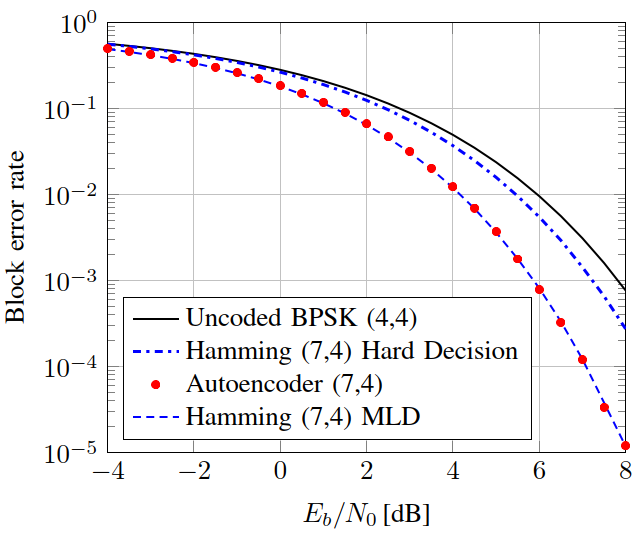
\includegraphics[width=0.8\linewidth]{figures/oShea_autoencoder_hamming_comp.PNG}
\end{center}
   \caption{Comparing block error rate for different SNRs of a learned autoencoder model with current state of the art, Hamming MLD. Taken from~\cite{oShea}}
\label{fig:oSheaAutoencoderHamming}
\end{figure}

The structure of this model is similar to an autoencoder, however with a noise layer in the middle. The encoder acts as the transmitter, the decoder as the receiver and the noise layer as the channel.

O'Shea and Hoydis then extended this to an adversarial network of many Rx Tx pairs competing for capacity. Next showing this is the same as one big MIMO NN which could be optimised in one go with a common or individual performance metric. The jointly learned metric outperformed a TS-QAM system across a range of SNRs as can be seen in \ref{fig:oSheaAutoencoderTsQam}.

\begin{figure}[t]
\begin{center}
   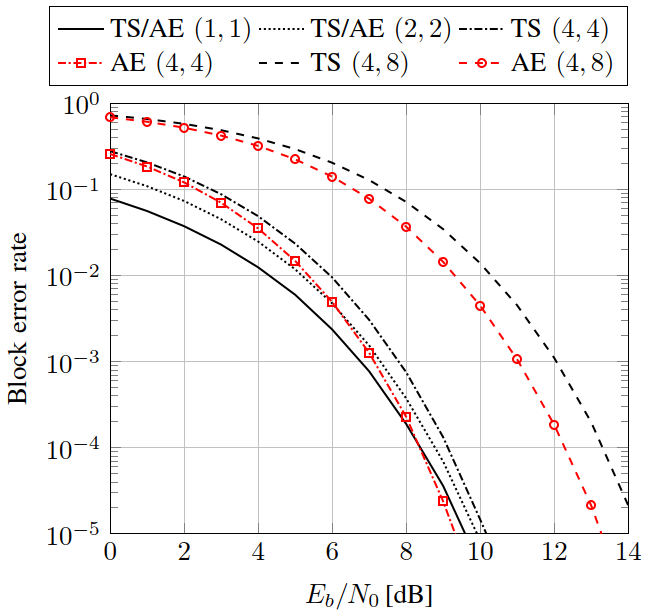
\includegraphics[width=0.8\linewidth]{figures/oShea_autoencoder_TS_QAM.PNG}
\end{center}
   \caption{Comparing block error rate for different SNRs of a learned autoencoder model with a TS-QAM system for a multi-agent communication system. From~\cite{oShea}}
\label{fig:oSheaAutoencoderTsQam}
\end{figure}

It should be noted though that autoencoders are notoriously bad with messages they haven't seen before, and consequently normally have to be trained using all the messages from the set of symbols $M = {1,...,M}$. This stops the method scaling to longer block lengths as there are $2^k$ possible messages in a block of lengths $k$ bits.

After this the authors added an RTN (radio transfer network). RTNs can perform a predefined correction algorithm, for example multiply by a complex number or convolute with a vector. This can be used as a way in incorporate some expert features into a learned system. This was integrated into the DLM for the end-to-end training process and consistently outperformed the normal NN. 

The learned system with added RTN's performance over a Rayleigh channel, with L=3 fading taps, can be seen in Figure \ref{fig:oSheaRtnRayleigh}. It should also be noted that not only did the RTN consistently outperform current state of the art, it also converged significantly faster than the normal autoencoder. This can be seen in Figure 10 of ~\cite{oShea}.

\begin{figure}[t]
\begin{center}
   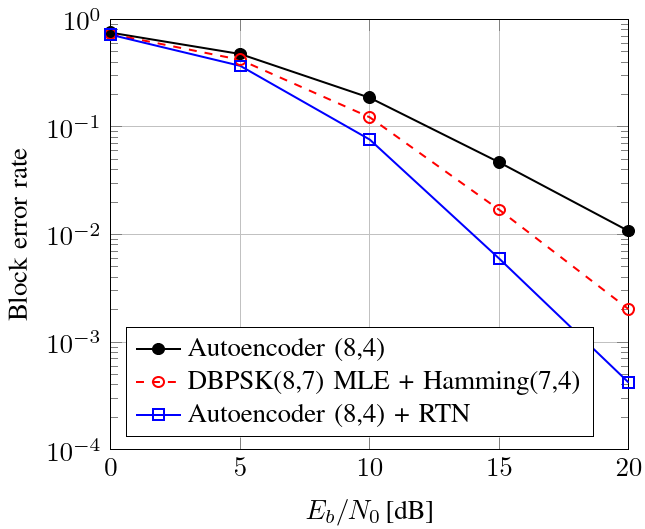
\includegraphics[width=0.8\linewidth]{figures/oShea_autoencoder_RTN_rayleigh_comp.PNG}
\end{center}
   \caption{BLER versus Eb/N0 for various communication schemes over a channel with L = 3 Rayleigh fading taps. Taken from~\cite{oShea}}
\label{fig:oSheaRtnRayleigh}
\end{figure}

Lastly they used a CNN (convolutional neural network) on raw coplex valued IQ (in-phase and quaternary) samples and found that it outperformed traditional classification techniques using expert features. This is consistent with the current trend that learned features are better than expert ones. 

\begin{figure}[t]
\begin{center}
   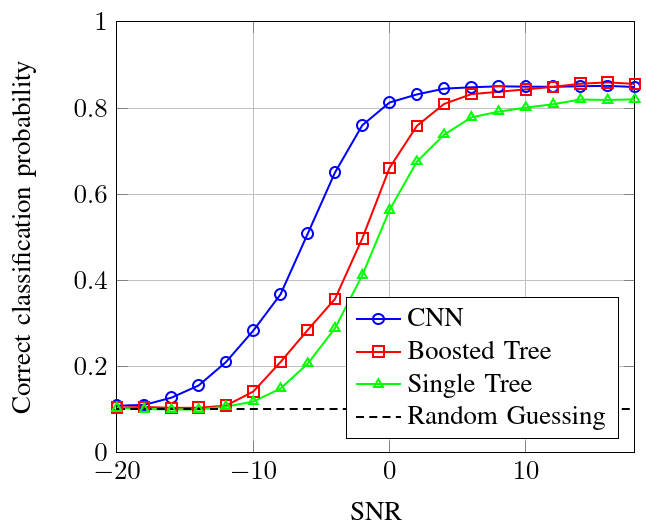
\includegraphics[width=0.8\linewidth]{figures/oShea_CNN_Rx_classification.PNG}
\end{center}
   \caption{Classification performance comparison versus SNR. Taken from~\cite{oShea}}
\label{fig:oSheaCnnRxClassification}
\end{figure}

In conclusion, comparison with traditional baselines showed extremely competitive BLER, however the inherent autoencoder lack of scalability makes this method impossible for any long block length communication. This method also requires a differentiable mathematical model for the channel, which is severely limiting as a big opportunity for this technology would be to learn optimal communication systems for channels we can't model. 

A very promising area though with potential uses of optical communications, where the channel impairments are highly non-linear and notoriously difficult to model and compensate for. Or alternatively unusual or complicated channels.

\subsection{End-to-end learning of communication systems without a channel model}

As highlighted in the conclusion of the O'Shea paper, normally if you use an autoencoder like a NN to learn a communication system you must have a differentiable channel model. This paper ~\cite{Aoudia}, written by Aoudia and Hoydis in April 2018, exclusively set out to remove the need for a channel model. 

They have a novel algorithm which gets around the problem. The algorithm iterates between the supervised training at the receiver and reinforcement learning (RL) at the transmitter. They showed it works as well as supervised methods using additive white Gaussian noise (AWGN) and using Rayleigh block-fading (RBF) channels. Their method converged slower on AWGN but faster on RBF as can be seen in Figure \ref{fig:AoudiaTrainingSpeeds}. This is the first step towards learning comms systems over any type of channel without and prior assumptions. 

\begin{figure}[t]
\begin{center}
   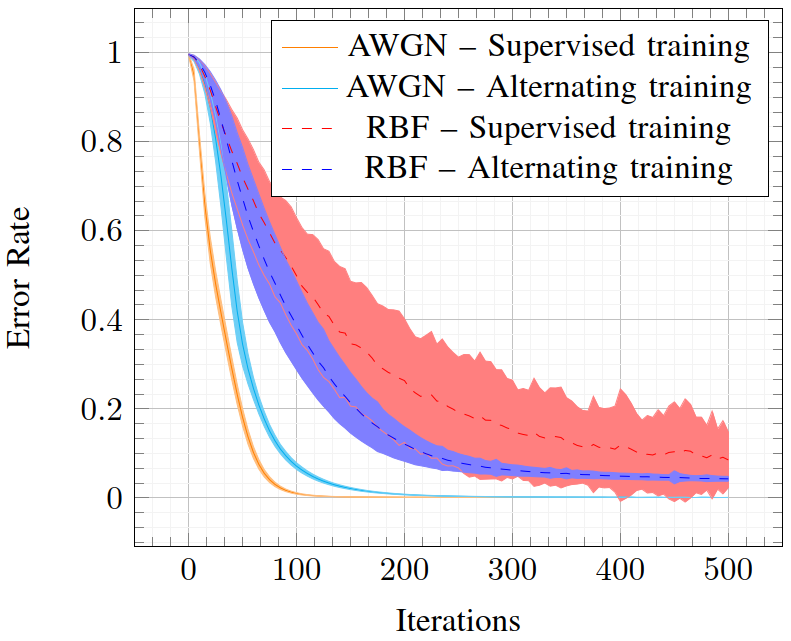
\includegraphics[width=0.8\linewidth]{figures/Aoudia_relative_training_speeds.PNG}
\end{center}
   \caption{Evolution of the error rate over the first 500 iterations. Taken from~\cite{Aoudia}}
\label{fig:AoudiaTrainingSpeeds}
\end{figure}

The reason this innovation is so important is that channels are normally black boxes, where only the inputs and outputs can be observed. 

The authors used a method called "Policy Learning", which is a subsection of RL. RL provides a theoretical foundation for obtaining an estimate of the gradient of an arbitrary loss function with respect to actions taken by an agent. In this case the agent is the transmitter and loss is performance metric provided by the receiver. This would mean knowledge of the channel model and instantaneous channel transfer function is not needed which allows them to train an autoencoder purely from observations. 

The "alternating training algorithm" trains the receiver first then the transmitter, alternating between training each side while keeping the parameters for the other side fixed. 

The receiver is trained using mini-batch stochastic gradient descent (SGD) as in other methods. For training the transmitter a random perturbation vector $\mathbf{w}$ is added. This is done for a whole batch of transmitted messages, these messages are then sent across the channel, and received as normal, the losses are calculated, and then transmitted back to the transmitter along a lossless channel. Finally a normal optimisation step is done using SGD where the loss-gradient is estimated using Equation 4 from ~\cite{Aoudia}. 

The authors found that the alternating method took longer to converge with for and AWGN channel and less time for an RBF channel than the supervised learning method. However it had the same end performance as the supervised method in both cases. This performance can be seen in Figures \ref{fig:AoudiaPerformanceAwgn} and \ref{fig:AoudiaPerformanceRbf}.

\begin{figure}[t]
\begin{center}
   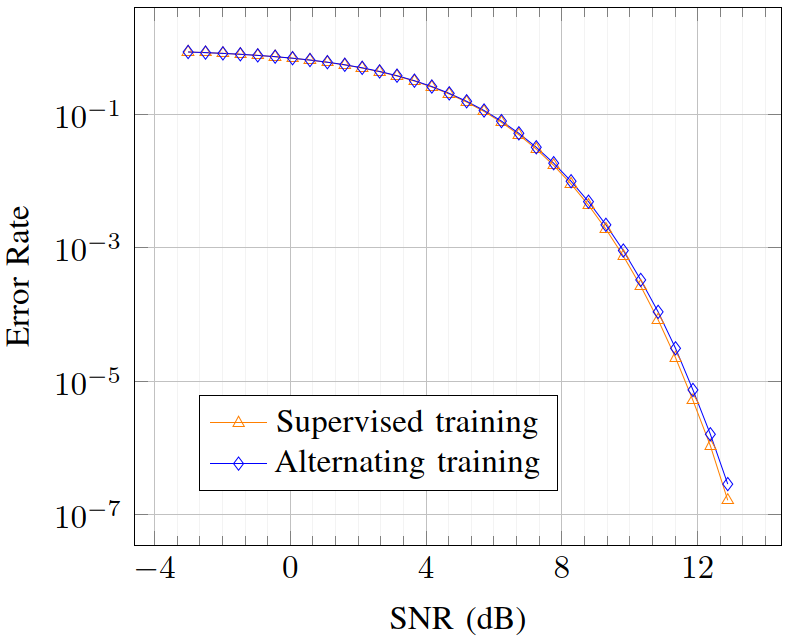
\includegraphics[width=0.8\linewidth]{figures/Aoudia_AWGN_performance.PNG}
\end{center}
   \caption{Alternative training vs autoencoder methods for AWGN Channel. Taken from~\cite{Aoudia}}
\label{fig:AoudiaPerformanceAwgn}
\end{figure}

\begin{figure}[t]
\begin{center}
   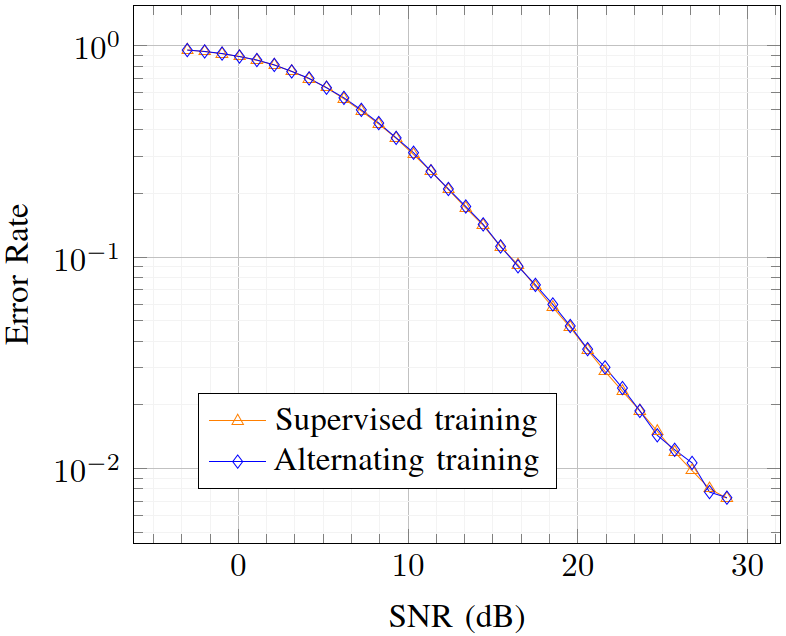
\includegraphics[width=0.8\linewidth]{figures/Aoudia_RBF_performance.PNG}
\end{center}
   \caption{Alternative training vs autoencoder methods for RBF Channel. Taken from~\cite{Aoudia}}
\label{fig:AoudiaPerformanceRbf}
\end{figure}

In conclusion they have shown they can get the same end performance to a fully supervised approach, but without needing a mathematical model of the channel, so it can therefore be applied to any type of channel without prior analysis. 
Although their algorithm currently requires an additional reliable channel during training to feedback losses from the receiver to the transmitter, this is still a huge step. It also does not solve help the problem of being restricted to short block lengths, and arguably makes it worse in the case of AWGN as the method takes longer to converge even with shorter block lengths.

However the importance of this step should not be underestimated. It allows learned communication systems to be used on channels which are either unknown, or too complex to model, which is arguably the biggest potential benefit of this technology. 

\subsection{A learning approach to wireless information and power transfer signal and system design}

This paper, written by Varasteh, Piovano and Clerkx has a slightly different focus. The previous two papers focused solely on achieving reliable communications with low error rates, this paper focuses on simultaneous wireless information and power transfer (SWIPT) using a nonlinear model, an autoencoder.

There is a fundamental trade-off between the information rate and the power rate and so the NNs are optimised using a joint loss function. 

The observed results were inline with previously theoretical results, particularly in that as you raise the demand for energy, the constellation diagram converges to one point a long way out along one of the axes, and the others closely clustering around the origin. However while this is what they would expect from the theory, it would not be possible to find these results theoretically or using numerical methods. So these found constellation, which can be found in Figure \ref{fig:VarastehConstellationDiagrams}, diagrams are novel and significant.

\begin{figure}[t]
\begin{center}
   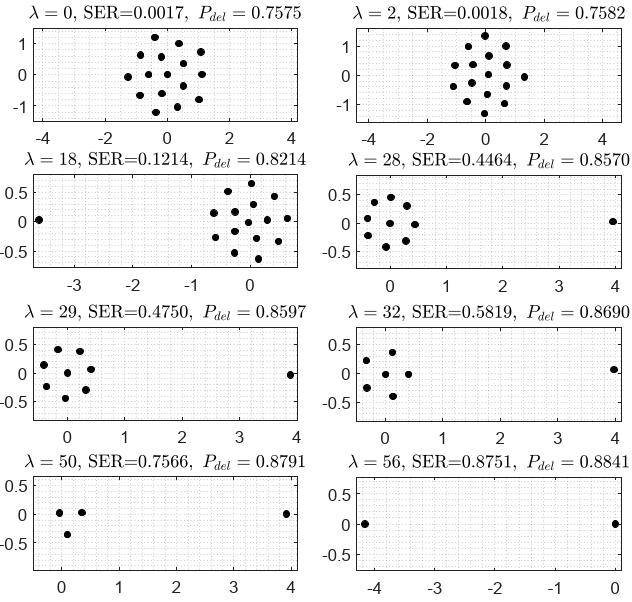
\includegraphics[width=0.8\linewidth]{figures/Varasteh_novel_constellation_diagrams.PNG}
\end{center}
   \caption{Representation of 16-symbols modulation for different values of λ (different information rate and power demand at the receiver) with SNR 20 dB. By increasing λ, the delivered power at the receiver increases. Taken from~\cite{Clerkx}}
\label{fig:VarastehConstellationDiagrams}
\end{figure}

To have a good SWIPT is essential to model the energy harvester with a high level of accuracy, which is an antenna and a rectifier with fundamentally non-linear characteristics. In the literature it is usually modelled linearly, using an NN allows it to be modelled non-linearly. 

Interestingly if you model the energy harvester (EH) linearly an analytical study found it prefers single carrier transmissions and also there is no trade-off between information and power transfer.  Whereas non-linear models favour multi-carrier transmission and have a trade-off between the two objectives.

Part of the motivation for a learned SWIPT system is that designing SWIPT signals and systems analytically is very cumbersome. 

The results were promising, the autoencoders and surpassed the performance of state-of-the-art algorithms.

The more channel symbols, the more DC power is received by the receiver. This is because to optimally transmit lots of power the transmitter favours the high probability information symbols around zero, and the low probability information symbols a long way from zero along on of the two axes. The more symbols you have the better it can fit the ideal pdf with all but one clustered symmetrically around the origin.

The symbols near the origin are called the information symbols, and the one which is far away from the origin is referred to as the power symbol.

Additionally the authors found that as the power demand increases, more of the channel symbols are sacrificed to increase the power delivery. Normally by mapping more of the information symbols to the origin. 

Another interesting observation by the authors was that the delivered power was "directly dependent on the channel input average power constraint". This means that two systems trained at the same SNR but with different transmitted powers would have different designs. However they left investigation of this aspect to another paper, along with investigation of the effect of block lengths on delivered power and making a model that features practical limitations of the rectenna non-linearity accurately.

This paper had some significant and completely new results, for instance the constellation diagrams would be impossible to find analytically because of the computational complexity of finding them. But in this paper they were able to find them using machine learning.

\subsection{Background communications theory}

\subsubsection{Type of fading}

Fading can be categorised into large or small scale, fast or slow and flat or frequency selective. Large scale fading is is due to path loss of signal as a function of distance ans shadowing by large objects, such as buildings and hills. Because of it's large spacial size it is usually frequency independent. 

Small scale fading is due to constructive and destructive interference of multiple signal paths between the transmitter and the receiver. This smaller spacial scale is of the order of the carrier wavelength and is therefore a function of frequency. 

In a learned communication system these factors could be taken account of, and as long as they were stationary an optimal communication system could be learned with no assumptions. Taking advantage of these factors is something a traditional communication would find more difficult.

To explain fast and slow fading we must first explain the meaning of coherence time. Coherence time is the time for which a channel is roughly constant as is shown by the diagram in Figure \ref{fig:coherence_illus}.

\begin{figure}[t]
\begin{center}
   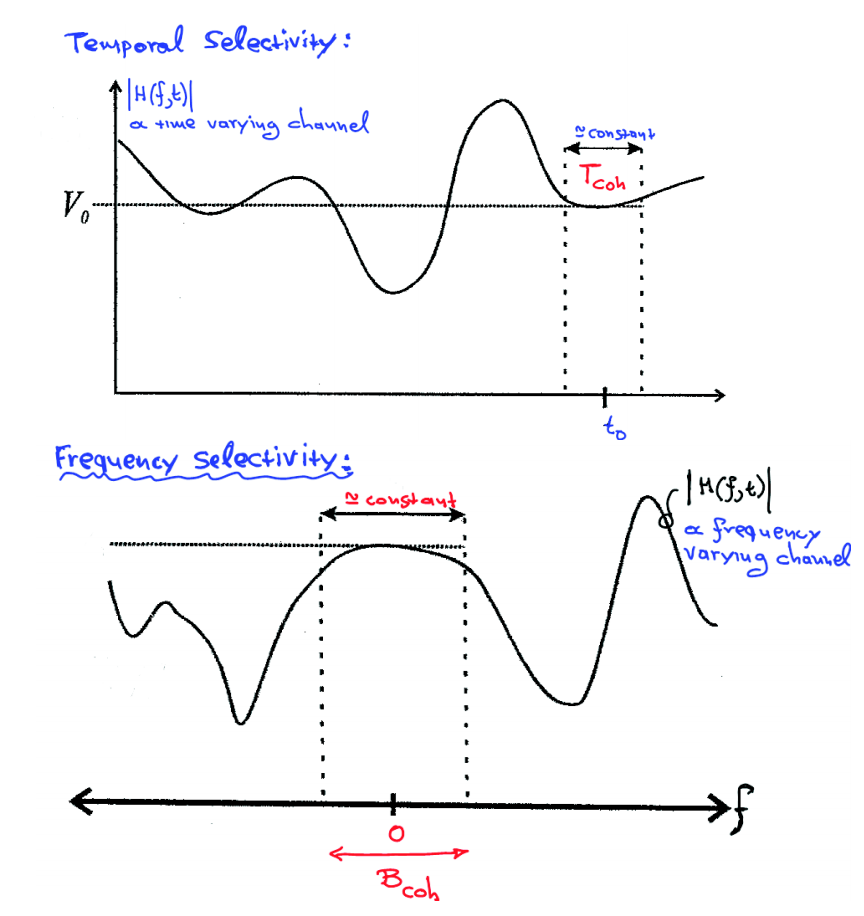
\includegraphics[width=0.8\linewidth]{figures/time_freq_coherence.PNG}
\end{center}
   \caption{A figure to demonstrate the meaning of coherence time ($T_{coh}$) and coherence bandwidth ($B_{coh}$) from~\cite{EE3CommsSystemsNotesL4}}
\label{fig:coherence_illus}
\end{figure}

There is little consensus as to exactly what fast and slow fading means~\cite{WirelessTextbookC2}. One interpretation is that a channel is fast fading if the coherence time is less than the delay requirement of the application, whereas is defined as slow fading if the coherence time is greater than the delay requirement of the application. 

However another definition which is shown in ~\cite{EE3CommsSystemsNotesL4} and is demonstrated in Figure \ref{fig:fast_slow_flat_freq_selec_fading} is that fading is fast if the time per channel symbol ($T_{cs}$) is greater than the coherence time ($T_{coh}$).

However defined either way the main difference between the two is that in fast fading channels you can transmit channel symbols over multiple channel fades, whereas in a slow fading channel you must transmit over that particular fade. This is either to satisfy the delay requirement of the application, or because your $T_{cs}$ is much shorter than your $T_{coh}$. Note that this behaviour depends on the channel characteristics (affects $T_{coh}$), the frequency (affects $T_{cs}$) and the application (sets the delay requirement).

\begin{figure}[t]
\begin{center}
   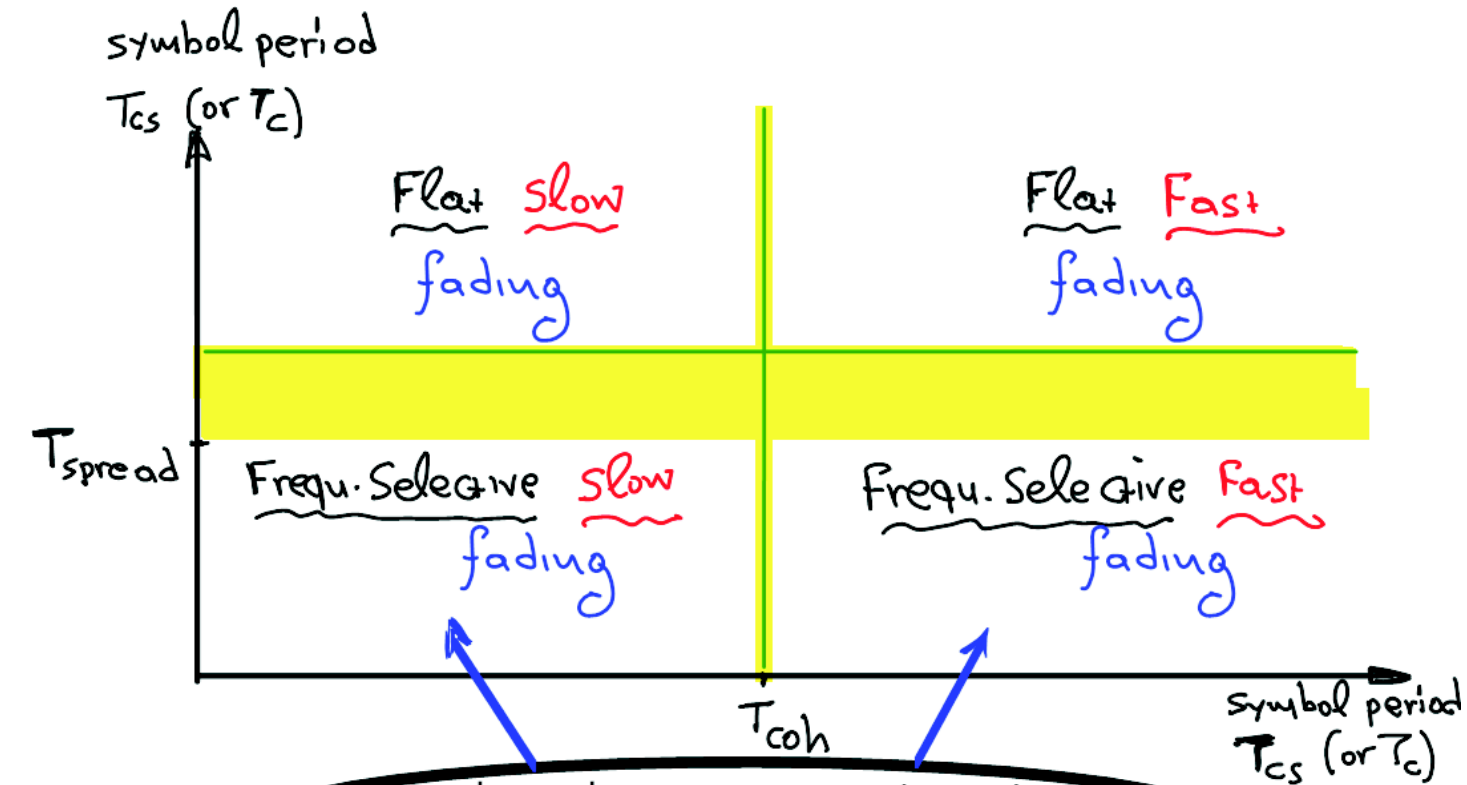
\includegraphics[width=0.8\linewidth]{figures/fast_slow_flat_freq_selec_fading.PNG}
\end{center}
   \caption{A figure showing how to classify a channel as fast/slow and flat/frequency selective fading taken from~\cite{EE3CommsSystemsNotesL4}}
\label{fig:fast_slow_flat_freq_selec_fading}
\end{figure}

For instance voice transmission usually has quite a low delay requirement of ${\sim}100$ms~\cite{WirelessTextbookC2}, but in different channels and transmitting at different frequencies could be either slow or fast fading.

Flat and frequency selective fading are similarly defined. Fading is flat if $T_{cs}$ is greater than $T_{spread}$. This means that the multi-paths for consecutive channel symbols will not overlap. Frequency selective fading is where the $T_{cs}$ is less than $T_{spread}$ and so multi-paths for consecutive channel symbols will overlap.

Faster, flatter fading is easier to design a communication system for. In the cases of frequency selective fading, which through the multi-paths depends on the environment, a learned communication system could learn an optimal system. This is another case of something which might be much more difficult to do analytically.

Because of these characteristics it seems likely that a learned communication system would be more suited to a very complex, but stationary environment. A good example of this may be an urban environment with many multi-paths. This would be very hard to model analytically and to do so would likely require assumptions which might make the solution sub-optimal. 

Whereas a learned system would avoid all these assumptions and learn the local optimum for that environment. However note that an urban environment may be too non-stationary for this method to work.

\subsubsection{Capacity and block lengths}

Shannon's capacity formula (Equation \ref{eqn:ShannonAwgnCapacity} taken from~\cite{WirelessTextbookC5}) describes a theoretical limit on the capacity of an AWGN channel as a function of SNR, however it does not specify a method of achieving said bound.

\begin{align}
    C_{AWGN} &= B.\log_2(1 + \frac{P}{\sigma^2})  \mbox{    (bits/sec)} \nonumber\\
    C_{AWGN} &= \frac{1}{2} \log_2(1 + \frac{P}{\sigma^2})  \mbox{    (bits/symbol)}
    \label{eqn:ShannonAwgnCapacity}
\end{align}

AWGN channels are now normally decoded using iterative decoding algorithms which are far faster but have very similar performance to maximum likelihood decoders, such as "turbo" and "low density parity check" (LDPC) codes~\cite{WirelessTextbookC5}. Using LDPC codes much lower error probabilities can be achieved by using longer block lengths~\cite{WirelessTextbookC5} to approach maximum theoretical capacity.

Another driver towards long block lengths is that Shannon's separation theorem proves, that if you separate the source encoding and the channel encoding, then this approach becomes theoretically optimal in the limit of infinitely long block lengths~\cite{ChannelEncodingOptimality}. This has led to most communication being done over very long block lengths. 

\begin{itemize}
    \item In OFDM if the block length is already very long then coding jointly across sub-carriers cannot increase the rate of reliable communication~\cite{WirelessTextbookC5}.
\end{itemize}

Capacity in fading channels must be thought of in a different way because whatever code is used the bit error probability ($p_e$) cannot be made arbitrarily small because the probability that the channel is in deep fade is non-zero~\cite{WirelessTextbookC5}. Deep fade is strong destructive interference which can result in temporary failure of communications due to a massive drop in channel SNR, so will cause an error whether the signal is encoded or not. It should also be noted that Equation \ref{eqn:FadingVsAwgnCapacity} always holds.

\begin{equation}
    C_{Fading} \leq C_{AWGN}
    \label{eqn:FadingVsAwgnCapacity}
\end{equation}

Because the probability of deep fade is non zero the strict sense capacity is zero. instead we find $C_{\epsilon}$ where $P(deep fade) < \epsilon$. 

However despite the fact we think about it differently the conclusion is the same for fast fading (time varying) channels. Because the code-words span several coherence periods the outage probability improves. This is because you can treat the different coherence periods as independent identically distributed (i.i.d) variables. By the law of large numbers their total variance will be lower. Extending this principle we like the block lengths to be long both to average out the effects of the Gaussian noise and the fluctuations of the channel. Hence the same conclusion, long block lengths.

Unfortunately using long block lengths has downsides. Firstly long block lengths give significant coding delays increasing latency even though they maintain throughput. Because of this in applications with tight delay constraints you may still get outage. 

Secondly for cases common in IoT applications where not much data needs to be send, long block lengths are not necessary and are impractical. 

The gains in longer block lengths are not as big for slower fading channels, so potentially this could be an area which a learned network of short block length communications systems could do well.

A problems with this though is that communication systems in slow fading channels often use feedback to the receiver to use \textit{channel inversion} to increase their capacity. Channel inversion is where the transmitter varies the input power to keep the receiver SNR constant~\cite{WirelessTextbookC5}. This can consume huge amounts of power though and so is not appropriate for IoT applications.

If the learned communication system could be adaptable or had a mechanism for feedback from the receiver to the transmitter then it might provide an alternative to channel inversion. Making communication in slow fading channels much more possible for IoT applications.

For all of these cases above where long block lengths are not feasible, short block lengths are necessary. However the coding techniques used for long block lengths have been shown to be sub-optimal~\cite{ShortBlockLengthNonOptimality} when used with short block lengths. Because of this there is a motivation to learn communications techniques specifically for this area.

\subsection{Additional notes}

This technique has great potential for providing flexible communication across highly non-linear, un-model-able or mathematically insoluble channels.

However it should be noted that in the case of non-stationary channels this method does not really have any potential without significant addition. The method could potentially be adapted to become adaptive, however this may be particularly difficult. This is because even in the most advanced form using the reinforcement learning you still require a noiseless channel between the receiver and the transmitter to communicate back what was received. 

This is fine if you are pre-training the network for a stationary channel you can train it with a noiseless channel temporarily. However if you are trying to update the weights online then you may lose significant capacity or use valuable resources such as frequency trying to transmit back the received bits to train the transmitter. 

This weakness for non-stationary channels is important as most wireless channels are highly non-stationary. 

\subsection{Analysis of competing products}

\begin{itemize}
    \item The first paper I am replicating claims there had not been much adoption of ML in commercial use ~\cite{oShea}. (Because of unspecified reasons "listed above")
\end{itemize}

The main commercial competition I have found is a start-up called DeepSig. One of it's two co-founders is Tim O'Shea, the co-author of the two founding papers on the subject of end-to-end learned communication systems. They currently have two commercial products OmniSIG and OmniPHY.

OmniSIG is a software package that allows training and monitoring of a communication system on a range of hardware devices. The package claims to often provide a 4-10 dB improvement and 10x reductions in computational complexity ~\cite{DeepsigOmnisig}. 

OmniPHY seems to be similar system however the information on their website is not very informative about what the product does, other than it learns a communication system, much like the OmniSig~\cite{DeepsigOmniphy}.

DeepSig appears to be in it's infancy, and I have been unable to find any other companies which are working in this area. It is not entirely surprising that DeepSig seems to be the first, as it's founder is one of the founders of the field. 

If I was producing a commercial application then such intellectually established competition would be quite worrying. So while I am only producing an academic report, it makes the research arguably less valuable as there is less chance for a company to get an early monopoly on the market. 

Due to the nature of the project being to reproduce the results of two existing papers, there are by definition competing papers. Alongside the two papers that I am reproducing ~\cite{oShea,Aoudia} there are also several existing papers which have applied similar methods to similar problems.

However few papers have learned a whole end-to-end communication system and the ones that have have been analysed in greater detail above.

\subsection{Analysis of necessary software tools}

I was asked to do my project in python and so this is why I chose python as the language to use. I am using python 3.6.8 because at the date of starting it is the latest version of python that supports Tensorflow and Keras. 

The main software tool that I will be using is Keras, with a Tensorflow backend. These are both open source machine learning libraries designed to make machine learning easier at a higher level. Allowing users to describe complicated networks in many fewer lines of code. The reason that I have chosen Keras is that the two paper's I am reproducing both specify that they used Keras~\cite{oShea,Aoudia}. 

\subsection{Analysis of necessary hardware}

The main hardware specification is what device do I need to be able to train and test my Keras model on. However any modern cpu core will be able to run Keras. It would be significantly faster to train and test on a graphical processing unit (GPU) as shown here~\cite{TensorflowBenchmarking}. But you can still run tensorflow and keras on a simple cpu, and this requirement will be satisfied by any modern laptop or desktop. 

The hardware I have chosen to use is my HP Spectre with an Intel I7 6500u. I have chosen to use this because of the convenience of it being my own laptop.

\FloatBarrier
\section{Implementation Plan}

This section will first go through the current progress of the project and then will cover the planned progress for the remainder of the project.

\subsection{Current progress}

Most of the first deliverable has been covered. An autoencoder based communication system that can be trained has been made, however it currently has a bug in that it is not using all of the possible communication symbols. This is suspected to be due to the regularisation method, however has not yet been fixed.

\subsubsection{Initial autoencoder model}

The development was started by building a simple autoencoder model in using Keras with a Tensorflow back-end. This was trained on the $M=2$ case with one hot encoded inputs and outputs. 

The model had a single dense layer transmitter, L2 normalisation layer, a Gaussian channel layer and a single dense layer receiver. This meant when tested after training over 1000 epochs on an input output relationship shown in Figure \ref{fig:CodeInitialOutput}.

\begin{figure}[t]
\begin{center}
   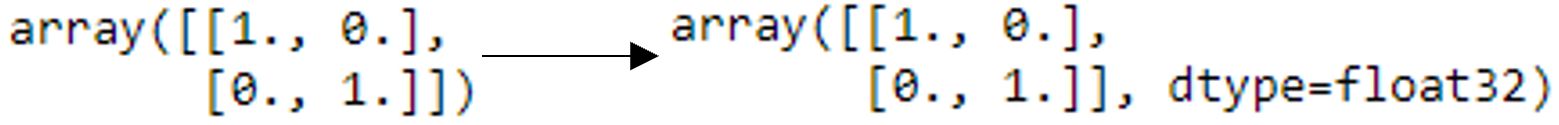
\includegraphics[width=0.8\linewidth]{figures/initial_ae_output.png}
\end{center}
   \caption{The input output of the initial autoencoder model during testing. }
\label{fig:CodeInitialOutput}
\end{figure}

\subsubsection{Adding noise at test time}

Clearly no noise has been added in the testing case. This is because the built in GaussianNoise layer in Keras is a training layer and so does not add noise if not in the training phase. 

To solve this problem a custom layer was added which adds noise both during training and testing as a channel model should. The code for this layer is shown in the appendix. This changed the input output relationship to the one shown in Figure \ref{}.

\begin{figure}[t]
\begin{center}
   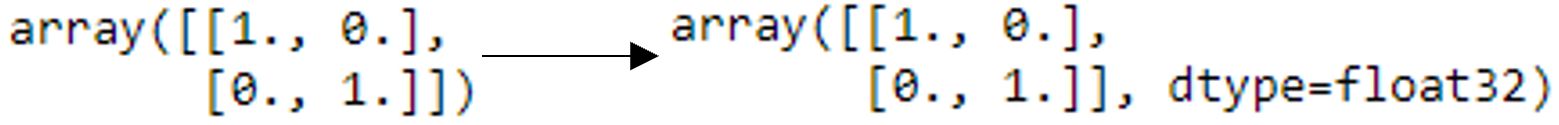
\includegraphics[width=0.8\linewidth]{figures/initial_ae_output.png}
\end{center}
   \caption{The input output of the autoencoder model with gaussian noise added at test time. }
\label{fig:CodeGaussianNoise2}
\end{figure}

\subsubsection{Adding a most likely symbol layer}

The output of the the receiver was a softmax layer, which gives an aposteri probability distribution for the symbols which were received. However at test time it is desirable to know the bit error rate, which required discrete bits.

To deal with this another custom layer was added to the output of the model which would take in the aposteri probability distribution and output the most likely symbol. An example of input output of this layer is shown in Figure \ref{fig:MostLikelySymbolLayer}.

\begin{figure}[t]
\begin{center}
   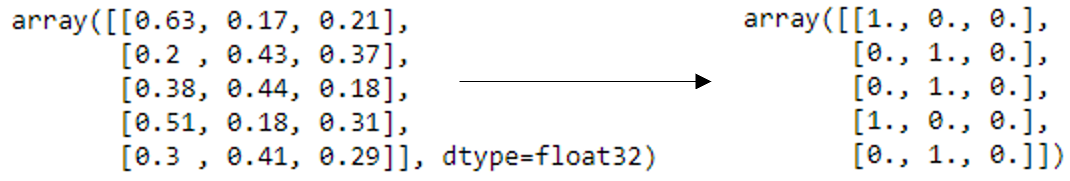
\includegraphics[width=0.8\linewidth]{figures/most_likely_symbol_io.PNG}
\end{center}
   \caption{The input output of the MostLikelySymbol layer. }
\label{fig:MostLikelySymbolLayer}
\end{figure}

This layer was originally written using a numpy based function, however this would not compile as part of the Keras model. This was probably because Keras could not differentiate the layer and so could not train the model. So a custom layer was written using Keras Tensorflow back-end functions.

\subsubsection{Making the channel symbols complex numbers}

Next the channel symbols were turned into complex numbers to represent the in-phase and quaternary sections of the transmitted signal. This required modifying the channel nodes of the model to have an extra dimension, which consequently forced a change in the regularisation layer.

This allowed channel symbols to now be meaningfully plotted. Some channel symbols are shown in Figure \ref{fig:WrongConstellationDiagram}.

\begin{figure}[t]
\begin{center}
   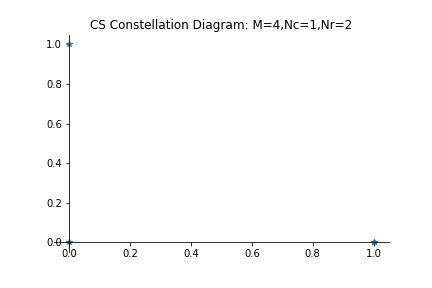
\includegraphics[width=0.8\linewidth]{figures/wrong_constellation_diagram.png}
\end{center}
   \caption{A constellation diagram produced by a trained model which is clearly wrong. }
\label{fig:WrongConstellationDiagram}
\end{figure}

In Figure \ref{fig:WrongConstellationDiagram} there are clearly only three constellation points, despite the fact there should be four. This is actually because the model has not learnt the $(1,1)$ channel symbol and so the first and third symbols have been mapped to the same channel symbol.

This is clearly as error, however it's source has not yet been found and dealt with. Another clear error about this constellation diagram is that the four points are mapped to only binary x and y coordinates. 

A normal constellation diagram would be expected to look more like what is shown in Figure \ref{fig:CommsSystemsConstelDiagEg}.

\begin{figure}[t]
\begin{center}
   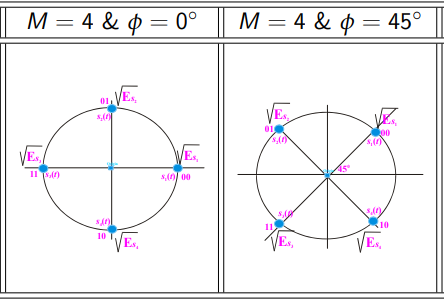
\includegraphics[width=0.8\linewidth]{figures/EE3-03_comms_systems_qpsk_constellation_diagram.PNG}
\end{center}
   \caption{An example of a correct QPSK constellation diagram taken from ~\cite{EE3CommsSystemsNotesL4}. }
\label{fig:CommsSystemsConstelDiagEg}
\end{figure}

In Figure \ref{fig:CommsSystemsConstelDiagEg} all of the points have an equal magnitude from the origin but are at different phases $90\deg$ apart to maximise separation for a given transmission power. 

This suggests that there is an error within the regularisation layer, however this bug is still in the process of being fixed. This is the current task which is being worked on, and when finished, after some minor modifications the model should be scale and so could be compared to BPSK and Hamming encoding to complete the first deliverable.

\subsection{Planned progress}
    
The first objective in the Gantt chart from Figure \ref{fig:GanttChart} has mainly been completed, however the other objectives all still need to be completed. This section will lay out a plan for when these objectives are expected to be completed and how long they are expected to take.

Finishing the autoencoder based model is expected to have been finished by the 13th of February, and the comparison of this model against current methods including DBPSK and Hamming encoding is expected to have been completed by the 15th of February. This is a hard deadline as there is a presentation to the project supervisors group on the morning of the 15th.

The following two deliverables have been given lots of time to complete despite not being expected to have large development content needed. This is because they span over the spring term which is very heavily loaded with coursework deadlines and an exam. Because of this the time allotted to specific deliverables decreases from the 26th of March. This will be the Easter holidays and so the author will only have two exams to revise for on top of the project, as opposed to the three coursework namodules and an exam module which are all in the spring term. 

The plan is to finish the fourth deliverable bt the 25th of April, so all the deliverables from the first paper by the end of the Easter holiday (25th of April), there will then be a weeks break to solely focus on exams. 

From after Easter there is a three week block to write the reinforcement learning model, which the project supervisor advised would be difficult, and compare it's performance to other models and current state of the art. This block finishes on the 26th of May.

There is a deadline for the first draft of the final report and abstract to be submitted on the 3rd of June, so the week between the 27th of May to the 3rd of June has been set aside purely for writing this first draft of the report. The following two and a half weeks until the submission deadline on the 19th of June have been set aside for continuing to write and then finish the report.

These estimates are not particularly optimistic, lots of extra time has been built into the estimates after the presentation on the 15th of February. The author plans to dedicate one day per week to the project, with specific goals for each day to ensure consistent progress with the project.

\begin{figure}[t]
\begin{center}
   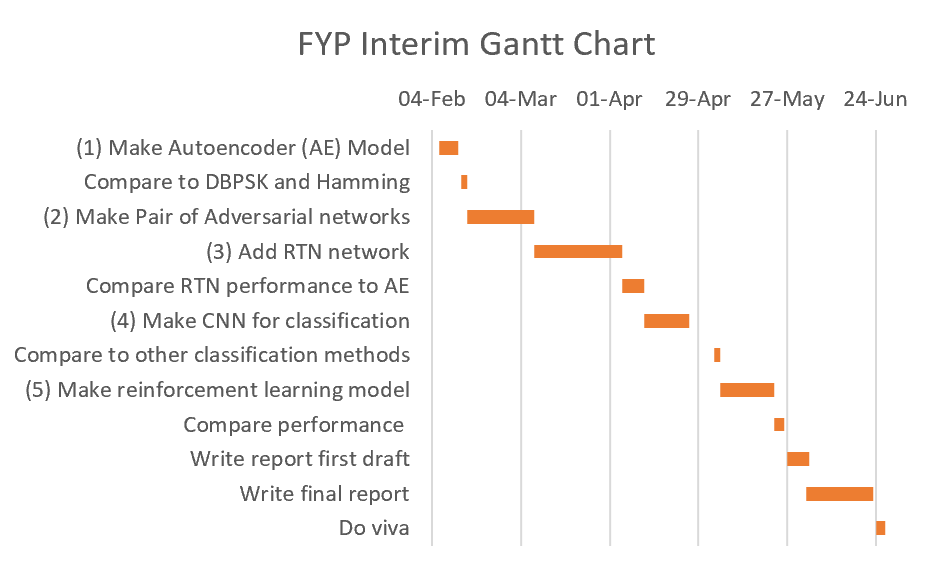
\includegraphics[width=0.8\linewidth]{figures/gantt_chart.png}
\end{center}
   \caption{A gantt chart showing planed progress through deliverables. }
\label{fig:GanttChart}
\end{figure}

\FloatBarrier
\section{Evaluation Plan}

The two main deliverables are to reproduce the results from two papers ~\cite{oShea,Aoudia}, so evaluation plan is relatively simple. The main deliverables are:

\begin{enumerate}
    \item Make an autoencoder model and compare it's performance to DBPSK and Hamming encoding across a range of SNRs.
    \item Produce a pair of adversarial networks both aiming to maximise their capacity, then show this is equivalent to a optimising one big NN with a joint loss function.
    \item Add an RTN network as a method for adding some expert features to the NN and then measure convergence speed compared to the autoencoder method and compare performance across a range SNRs.
    \item The last deliverable in the O'Shea paper is comparing the performance of a CNN relative to other receiver classification methods across a range of SNRs.
    \item Reproduce the model from ~\cite{Aoudia} which uses the alternate training method. The compare the performance of this model against current state of the art and the autoencoder method across a range of SNRs for an AWGN and an RBF channel.
\end{enumerate}

Assessing the completeness of the above deliverables should be relatively simple, in that the results produced can be compared with the results that are being reproduced, and if they are the same then the deliverable is complete.

The author also recently found a github repository which reproduces the results from the first (O'Shea \etal) paper. Consequently the code from this repository can be used to verify this project's code works, potentially by first producing a testbench which can then be used to test all subsequent models work. It should be noted though that this repository is written using a different python library to the library (Keras) that must be used for this project so it cannot be copied.

When the program has been written the github repository can be used to produce a testbench, which can then bus used to test the program. However before this can be done the legitimacy of the source code must be verified and so the results of the testbench must be compared to those of the report which is being reproduced.

The first repository was discovered by accident, but after brief research, a repository for the second paper ~\cite{Aoudia} has not been found. For this paper comparing the results of the code to the graphical results in the paper will have to be sufficient as there are no numerical results provided.

Some extra comparisons that is aimed to be completed on top of the main deliverables are comparing the learned systems to Shannon's theoretical capacity limit and current state of the art codes such as turbo and LDPC codes for an AWGN channel.

Additional comparisons which are aimed to be done are comparing the learned networks and current state of the art across common fading channels such as Rayleigh and Ricean channels across a range of type of fading, large scale or small scale, fast or slow, flat or frequency selective. After which it is aimed to do the same for some rare or hard to model channels. These are where the learned communication system should have the biggest advantage and so it should be interesting to see if they can deliver on their potential.

If the main deliverables are finished then further research will be started by investigating adding an RTN layer to the receiver of the reinforcement learning model. The project supervisor had stated that
if section is reached then he will decide which of the two areas is most current between reinforcement learning and SWIPT and further research will be continued into this area. The details of these deliverables are described in the project specification, however as these will be new areas a different method of evaluating the success and validity of the results.

The code I have written for previous deliverables will be used, producing results for learned systems and current state of the art, to give ball park figures to check the code is roughly working. Then each small function will be tested thoroughly to ensure the overall system is working. 

It is hard to predict whether the results make sense, but they will be checked against theoretical estimations and if there is still uncertainty the project supervisors will be consulted. 

\FloatBarrier
\section{Ethical, Legal and Safety Plan}

\subsection{Ethical considerations}

One interesting ethical consequence of this project is that, if this technology becomes very successful and so very competitive with or superior to current state of the art communications systems, it could reduce the number of jobs for communications engineers. 

If it was possible to just set up a generic transmitter and receiver, then let them train for their environment and then just have them run at optimal performance, there there would not a need for communications engineers to design systems.

While this would be bad for current communications engineers, it would lead to greater productivity and efficiency by companies which would contribute to greater economic growth, which would then trickle back down. So while it may be bad for a minority, it should be better for the majority, therefore overall it is ethically alright. 

However other than this there are no significant ethical implications of this project.

\subsection{Legal consideration}

\subsubsection{Infringing patents}

A search was performed on Espacenet, which was found by direction from the UK government website. This seach of Espacenet was to see if there were any parents which this project might be infringing.

Patents were searched for using related key words, however no patents of similar ideas were found. Consequently the project is likely safe from infringing any patents. If there were any significant commercial consequences of this report then a more thorough search could be carried out through a patent attorney, however this would be expensive and is unlikely to be needed.

The legal alternative to patents for protection of intellectual property is referred to as a "trade secret". However these are only legally binding for company employees who have signed a non disclosure agreement (NDA), or if someone is accessing the information either when they do not have the permission to access it, or they are receiving it from someone who doesn't have the permission to access it. 

Trade secrets become non-binding once the information is publicly available, so as the papers that this paper is reproducing are publicly available it cannot be infringing any trade secrets that the author is unaware of. 

\subsubsection{Use of data}

The other potential legal concern for a project of this type is potentially using someone's data inappropriately while training a machine learning model. For the first part of this project this isn't possible as the model involves training an autoencoder-like model. 

In this method the desired output is the initial input, and that input is any one of the potential combinations of n binary bits. This is where n is the block length. Hence there is no involvement of non-self-generated data and so can be no illegal use of someone else's data.

In the last of the main deliverables where would be developing the reinforcement learning model which could be trained on any samples from any channel there is marginally more of a risk of this.

To counter this risk it will be made sure that these samples are sourced from publicly available sources, so people who have contributed to it will have signed that they consented to having their data collected. 

However it should be made clear that it should be more or less impossible to decode the information that people were sending across a channel from the channel interference samples. To ensure there can be no accusations of this the data and model will be kept private, results will not be shared publicly and there will be no inspection of the channel interference.

\subsubsection{Licences of used libraries}

The Keras library has an MIT lisence, which means that users have the right to "use, copy, modify, merge, publish, distribute, sublicense, and/or sell copies of the Software" as long as a copyright notice is place in the code. 

To ensure that this is abided by, if the software from this project is published then Keras will be acknowledged and referenced. Additionally the copyright stamp will be included in the code if it is published. 

\subsection{Safety Plan}

Firstly it should be stated that compared to hardware projects there are no really pressing safety issues. However the relevant safety issues are assessed in Table \ref{tab:RiskAssessment}. 
%The sources of the first three rows of information in the "Mitigation Plan" section of the table are ~\cite{NhsRepetitiveStrainInjury, EyeStrain, NhsCorrectChainPosture} respectively.

% \FloatBarrier

\begin{table*}[!htbp]
\resizebox{\textwidth}{!}{
\centering
{\small \hfill{}
\small
\begin{tabular}{|p{1.2cm}|p{1.5cm}|p{1.3cm}|p{1.2cm}|p{7cm}|}
\hline
\textbf{Risk}                  & \textbf{Potential Cause}          & \textbf{Likelihood (/5)} & \textbf{Potential Harm (/5)} & \textbf{Mitigation Plan}                                                                                                                                                                                                                                                       \\ \hline
Repetitive strain injury (RSI) & Excessive use of laptop           & 4                        & 1                           & I will take regular breaks every 20-60 minutes. If I get RSI then I will identify what movement is causing it and stop this movement. I will also treat it with hot and cold treatment, rest and anti-inflammatories like ibuprofen.  {[}{]}                                    \\ \hline
Eye Strain                     & Excessive use of laptop           & 4                        & 2                           & To avoid straining my eyes I will try to work with adequate, but not too bright, lighting at all times, and will rest my eyes every twenty minutes. I will also try to keep the screen approximately 20-24 inches away from my eyes and 10-15 inches below my eye line. {[}{]} \\ \hline
Back Pain                      & User's poor posture               & 2                        & 2                           & I have set my chair at my work station up according to this NHS guide {[}{]} and a will make more effort to sit with correct posture to avoid back pain which might prevent me from working.                                                                                   \\ \hline
Trip Hazards                  & Often work with laptop plugged in & 1                        & 2                           & I will make sure that my charger lead is as short as possible and does not stretch across any areas where people regularly walk.                                                                                                                                               \\ \hline
Electric shocks                & Often work with laptop plugged in & 1                        & 5                           & I will be careful when plugging and unplugging my laptop to avoid shocking myself.                                                                                                                                                                                             \\ \hline
Fires                          & Often work with laptop plugged in & 1                        & 5                           & I will not leave my laptop plugged in unsupervised. I have also checked that my laptop charger has been PAT tested and so I think I have taken reasonable steps.                                                                                                               \\ \hline
\end{tabular}
}}
\caption{Risk assessment in table form}
\label{tab:RiskAssessment}
\end{table*}

\FloatBarrier
\section{Analysis and Design}

\FloatBarrier
\section{Implementation}

\FloatBarrier
\section{Testing}

\FloatBarrier
\section{Results}

\FloatBarrier
\section{Evaluation}

\FloatBarrier
\section{Conclusions and Further Work}

\FloatBarrier
\appendix
\section{Appendix}


{\small
\bibliographystyle{ieeetr}
\bibliography{egbib}
}

\end{document}
